For the simulation results we looked into a few different \textcolor{red}{things}.

\subsection{Effect of different ordering}
We wanted to see how big of an impact has the order of the tasks. That is why we looked for the best order for the recipe for goulash, and the worst one. This means the one that is done the quickest and the one that takes the longest.
The following results are done with two cooks and time randomness.

\begin{verbnobox}[\fontsize{10pt}{10pt}\selectfont]
BEST ORDER: 168, 
[cutting meat, peeling potatoes, heating water, cutting onions, cooking meat, 
cooking potatoes, frying onions, cooking everything]
\end{verbnobox}

\begin{verbnobox}[\fontsize{10pt}{10pt}\selectfont]
WORST ORDER: 253,
[cutting onions, cutting meat, heating water, cooking meat,
 frying onions, peeling potatoes, cooking potatoes, cooking everything]
\end{verbnobox}

We can see that the difference in duration is 55 units of time, which is not small. 
This happens due to probalistic duration of time, but even without that, the difference would still be 30 units. The reason for that is the order of the first few tasks, 
which have to be done before cooking potatoes and cooking everything. If they are not done in the best order, the simulation has to wait for a task to be finished before doing anything new. 

\begin{figure}[H]
    \centerline{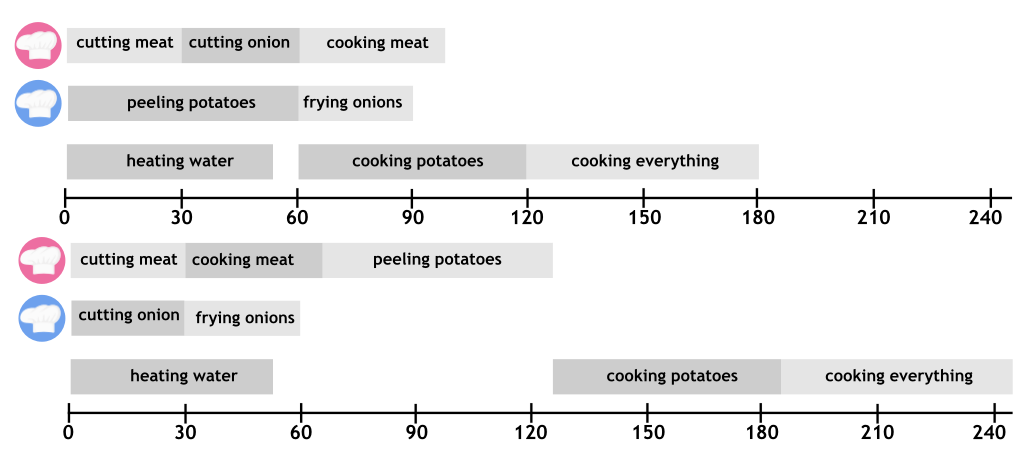
\includegraphics[scale=.4]{/Users/lanar/Documents/Cooking-model/Documentation/images/recipes_order.png}}
    \caption{The best and worst order of tasks.}
    \label{fig3}
\end{figure}

After seeing the difference an order of tasks can have, we were interested to see what are all possible durations of the recipe and which are the most common. 
In the histogram below we can make out that most of the time the recipe is completed in between 179 to 184 units of time, this suggests the order was similar to the best order as seen above, with just some different permutations of the first few tasks.

\begin{figure}[H]
    \centerline{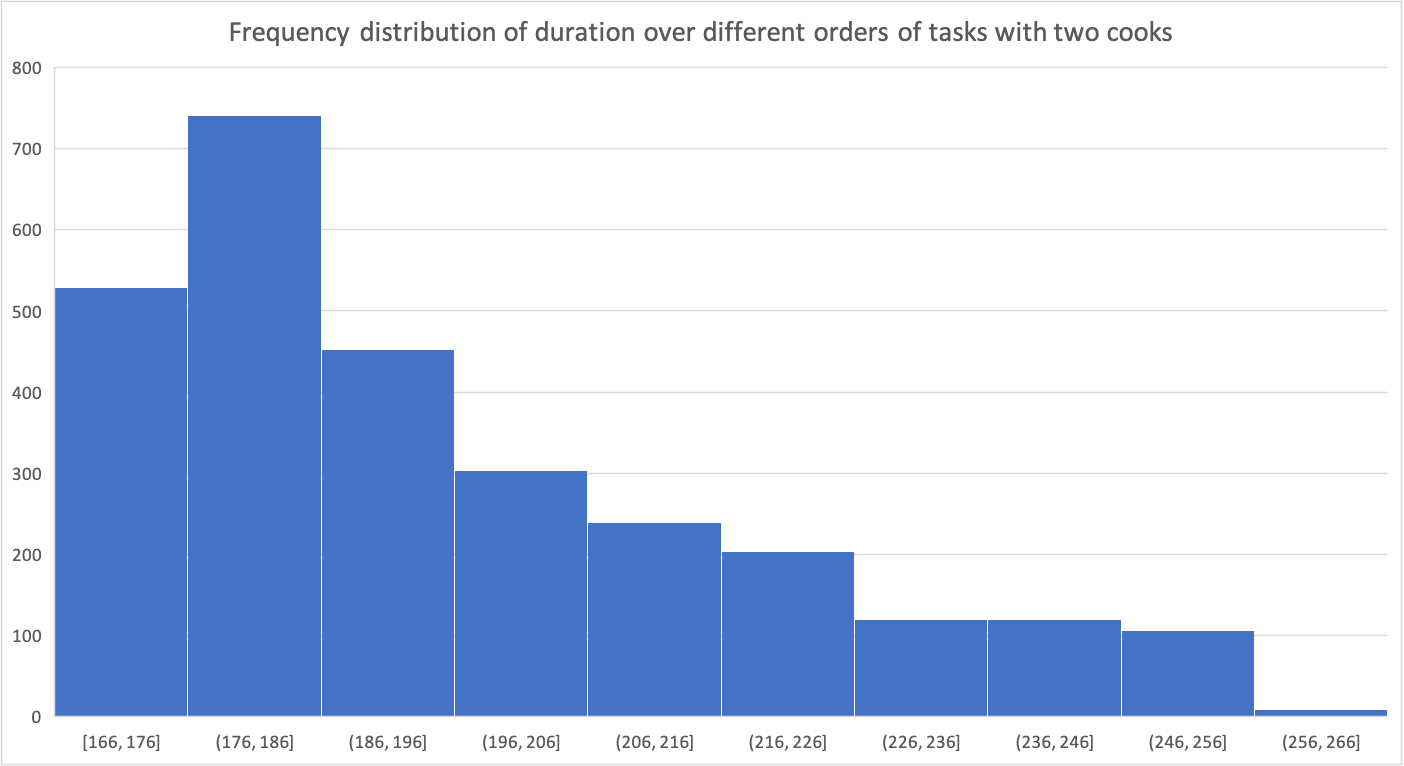
\includegraphics[scale=.5]{/Users/lanar/Documents/Cooking-model/Documentation/images/graph_duration.png}}
    \caption{All possible durations of the recipe with two cooks, devided into groups by time interval 5 units.}
    \label{fig4}
\end{figure}

We also did the same calculations for just one cook, but got a somewhat different distrubution, with most of the odrers gathered in the middle. In this case the different durations were only a result of probalistic time assignment, 
because when we ran the stohastic model, we only got one option of duration which is 251. This can be seen on the graph where most orders are between 243 to 248 units of time. 

\begin{figure}[H]
    \centerline{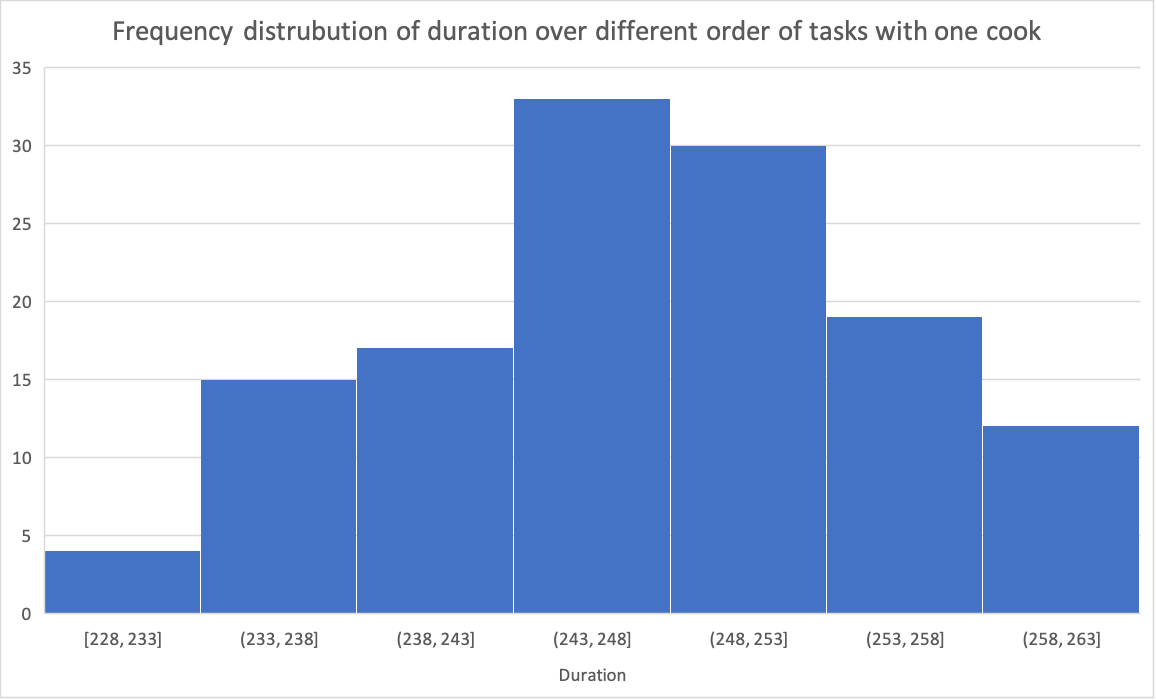
\includegraphics[scale=.5]{/Users/lanar/Documents/Cooking-model/Documentation/images/graph_duration1.png}}
    \caption{All possible durations of the recipe with one cook, devided into groups by time interval 5 units.}
    \label{fig5}
\end{figure}

\newpage
\subsection{Recipe comparison to cook book}
For our second dish we decided to do potato salad. We found a recipe in a cook book and adjusted it to our program. We wanted to test if the calculated optimal order for one cook matches the order in the cook book.
Here we can see the two orders:

\begin{verbnobox}[\fontsize{10pt}{10pt}\selectfont]
    COOK BOOK:                                  OPTIMAL ORDER:
    - cooking potatoes                          - cooking potatoes
    - cooking eggs                              - cooking eggs
    - cutting pickles                           - cutting onions
    - cooling eggs                              - make dressing
    - cutting onions                            - cutting pickles
    - peeling eggs                              - cooling eggs
    - cutting eggs                              - peeling eggs
    - peeling potatoes                          - peeling potatoes
    - cuttting potatoes                         - cutting potatoes
    - make dressing                             - cutting eggs
    - mixing enerything                         - mixing enerything
\end{verbnobox}

We can see that the two orders don not differ much. Some tasks are done in different order, but those are mainly interchangable. One different thing is when the dressing is done. 
But this is because in real life you would want it to be freshly done before completing the salad, and our program does not take this into account. 

\subsection{Different number of resources}
Lastly we focused on the number of resources to see if it really has that big of an effect on duration. 
We ran the program 5 times for each number of cooks and took the average of the optimal time. We gave the other resources a high enough quantity so that it won't effect the duration.
These are the graphs we got.

\begin{figure}[H]
    \centering
    \begin{minipage}{.5\textwidth}
      \centering
      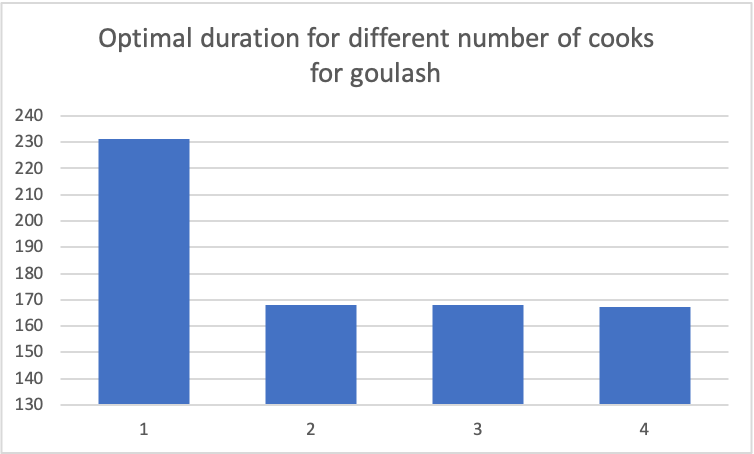
\includegraphics[width=.9\linewidth]{/Users/lanar/Documents/Cooking-model/Documentation/images/optimal_durationG.png}
      \caption{Duration of recipe goulash with \\ different number of cooks}
      \label{fig6}
    \end{minipage}%
    \begin{minipage}{.5\textwidth}
      \centering
      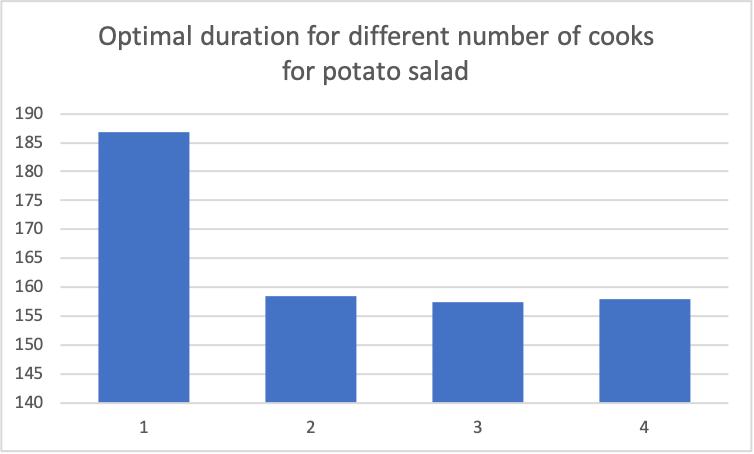
\includegraphics[width=.9\linewidth]{/Users/lanar/Documents/Cooking-model/Documentation/images/optimal_durationS.png}
      \caption{Duration of recipe potato salad with different number of cooks.}
      \label{fig7}
    \end{minipage}
\end{figure}

As you can see there is only a difference when using one or two cooks, after that you can use as many as you want, but the duration won't change. 
This is because the tasks in our recipes already have an order in which they have to be done and even if you have another cook, he still has to wait for the other task to finish. 
To test our program we decided to make another recipe, where we tried to do it so, that a different number of cooks will have a bigger effect.

\begin{figure}[H]
    \centerline{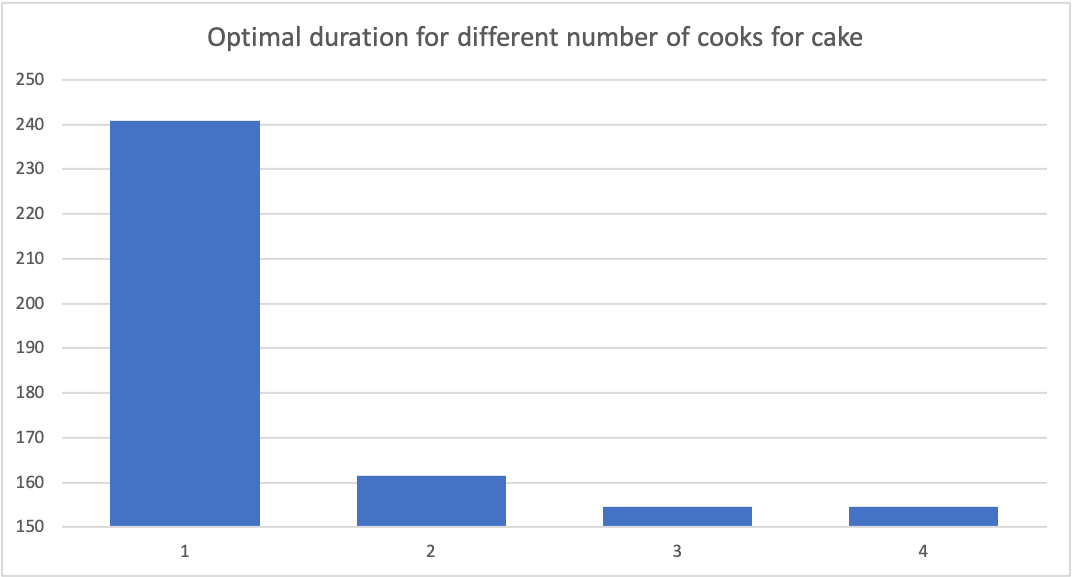
\includegraphics[scale=.5]{/Users/lanar/Documents/Cooking-model/Documentation/images/graph_durationC.png}}
    \caption{Duration of recipe cake with different number of cooks.}
    \label{fig8}
\end{figure}

These are the results we got with implementing the recipe of baking a cake. We wanted to have more independant tasks and less strict prior ordering. 
In this recipe you have to do a lot of tasks independantly and then there is just a few tasks that combine all of them. This way you can see a difference 
between one, two and three cooks, but when it comes to four, the duration still remains the same. FUrthermore the difference was very small, only 6 time uhnits. This brings us to the conslusion that with every recipe 
there will be a point where the number of cooks doesn't matter anymore. 

%ADD GRAPH FOR POTATO SALAD, ONLY ONE OF EVERY RESOURCE

Besides observing the effect of the number of cooks, we did the same for other resources. Here you can see the duration for making goulash when having:
\begin{itemize}
    \item double of everything: 181
    \item only one pan: 191
    \item only one knife: 181
\end{itemize}

This is because in the optimal recipe two knives are never used at the same time, while the pan is used for cooking the meat and frying the onions which is done at the same time. 

\begin{figure}[H]
    \centerline{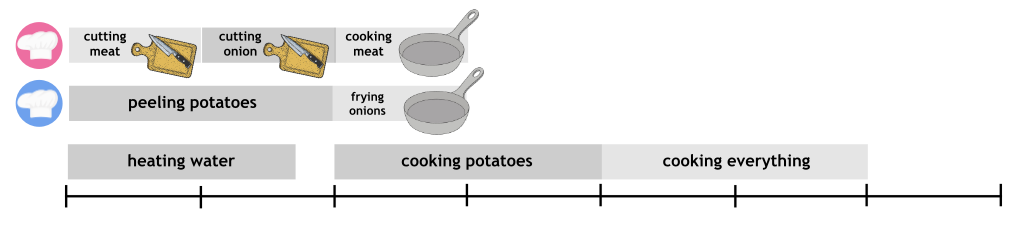
\includegraphics[scale=.4]{/Users/lanar/Documents/Cooking-model/Documentation/images/resources.png}}
    \caption{Use of pan and knife in the optimal order of the recipe goulash.}
    \label{fig9}
\end{figure}
